%package list
\documentclass{article}
\usepackage[top=3cm, bottom=3cm, outer=3cm, inner=3cm]{geometry}
\usepackage{multicol}
\usepackage{graphicx}
\usepackage{url}
\usepackage{hyperref}
\usepackage{array}
\newcolumntype{x}[1]{>{\centering\arraybackslash\hspace{0pt}}p{#1}}
\usepackage{natbib}
\usepackage{pdfpages}
\usepackage{multirow}
\usepackage[normalem]{ulem}
\useunder{\uline}{\ul}{}
\usepackage{svg}
\usepackage{xcolor}
\usepackage{listings}
\lstdefinestyle{ascii-tree}{
    literate={├}{|}1 {─}{--}1 {└}{+}1 
  }
\lstset{basicstyle=\ttfamily,
  showstringspaces=false,
  commentstyle=\color{red},
  keywordstyle=\color{blue}
}
%\usepackage{booktabs}
\usepackage{caption}
\usepackage{subcaption}
\usepackage{float}
\usepackage{array}

% Comment
\usepackage{verbatim}

\newcolumntype{M}[1]{>{\centering\arraybackslash}m{#1}}
\newcolumntype{N}{@{}m{0pt}@{}}


%%%%%%%%%%%%%%%%%%%%%%%%%%%%%%%%%%%%%%%%%%%%%%%%%%%%%%%%%%%%%%%%%%%%%%%%%%%%
%%%%%%%%%%%%%%%%%%%%%%%%%%%%%%%%%%%%%%%%%%%%%%%%%%%%%%%%%%%%%%%%%%%%%%%%%%%%
\newcommand{\itemEmail}{rzapata@unsa.edu.pe}
\newcommand{\itemStudent}{Reyser Julio Zapata Butron}
\newcommand{\itemCourse}{Tecnología de Objetos}
\newcommand{\itemCourseCode}{1703240}
\newcommand{\itemSemester}{VI}
\newcommand{\itemUniversity}{Universidad Nacional de San Agustín de Arequipa}
\newcommand{\itemFaculty}{Facultad de Ingeniería de Producción y Servicios}
\newcommand{\itemDepartment}{Departamento Académico de Ingeniería de Sistemas e Informática}
\newcommand{\itemSchool}{Escuela Profesional de Ingeniería de Sistemas}
\newcommand{\itemAcademic}{2024 - B}
\newcommand{\itemInput}{26 septiembre 2024}
\newcommand{\itemOutput}{03 octubre 2024}
\newcommand{\itemPracticeNumber}{02}
\newcommand{\itemTheme}{Punteros en C++}
\newcommand{\itemPracticeDuration}{02 horas}
%%%%%%%%%%%%%%%%%%%%%%%%%%%%%%%%%%%%%%%%%%%%%%%%%%%%%%%%%%%%%%%%%%%%%%%%%%%%
%%%%%%%%%%%%%%%%%%%%%%%%%%%%%%%%%%%%%%%%%%%%%%%%%%%%%%%%%%%%%%%%%%%%%%%%%%%%

\usepackage[english,spanish]{babel}
\usepackage[utf8]{inputenc}
\AtBeginDocument{\selectlanguage{spanish}}
\renewcommand{\figurename}{Figura}
\renewcommand{\refname}{Referencias}
\renewcommand{\tablename}{Tabla} %esto no funciona cuando se usa babel
\AtBeginDocument{%
	\renewcommand\tablename{Tabla}
}

\usepackage{fancyhdr}
\pagestyle{fancy}
\fancyhf{}
\setlength{\headheight}{30pt}
\renewcommand{\headrulewidth}{1pt}
\renewcommand{\footrulewidth}{1pt}
\fancyhead[L]{\raisebox{-0.2\height}{
\includegraphics[width=3cm]{img/logo_episunsa.png}}}
\fancyhead[C]{\fontsize{7}{7}\selectfont	\itemUniversity \\ \itemFaculty \\ \itemDepartment \\ \itemSchool \\ \textbf{\itemCourse}}
\fancyhead[R]{\raisebox{-0.2\height}{
\includegraphics[width=1.2cm]{img/logo_abet}}}
\fancyfoot[L]{\itemStudent}
\fancyfoot[C]{\itemCourse}
\fancyfoot[R]{Página \thepage}

% Estilos del Código
\usepackage{listings}
\usepackage{color, colortbl}
\definecolor{dkgreen}{rgb}{0,0.6,0}
\definecolor{gray}{rgb}{0.5,0.5,0.5}
\definecolor{codebackground}{rgb}{89, 0.97, 0.90}
\definecolor{tablebackground}{rgb}{0.8, 0, 0}

\lstset{
  language=C++,                  
  basicstyle=\ttfamily\footnotesize,
  keywordstyle=\color{blue},     
  commentstyle=\color{dkgreen},    
  stringstyle=\color{red},       
  backgroundcolor= \color{codebackground},
  numbers=left,                  
  numberstyle=\tiny\color{gray},
  stepnumber=1,                  
  numbersep=5pt,                
  showspaces=false,              
  showstringspaces=false,      
  showtabs=false,                
  frame=single,                  
  captionpos=b,                  %
}

\begin{document}
	\vspace*{10px}
	
	\begin{center}	
		\fontsize{17}{17} \textbf{ Informe de Laboratorio \itemPracticeNumber}
	\end{center}

 %% TABLA %%
 
	\centerline{\textbf{\Large Tema: \itemTheme}}

	\begin{flushright}
		\begin{tabular}{|M{2.5cm}|N|}
			\hline 
			\rowcolor{tablebackground}
			\color{white} \textbf{Nota}  \\
			\hline 
			     \\[30pt]
			\hline 			
		\end{tabular}
	\end{flushright}	

	\begin{table}[H]
		\begin{tabular}{|x{4.7cm}|x{4.8cm}|x{4.8cm}|}
			\hline 
			\rowcolor{tablebackground}
			\color{white} \textbf{Estudiante} & \color{white}\textbf{Escuela}  & \color{white}\textbf{Asignatura}   \\
			\hline 
			{\itemStudent \par \itemEmail} & \itemSchool & {\itemCourse \par Semestre: \itemSemester \par Código: \itemCourseCode}     \\
			\hline 			
		\end{tabular}
	\end{table}		
	
	\begin{table}[H]
		\begin{tabular}{|x{4.7cm}|x{4.8cm}|x{4.8cm}|}
			\hline 
			\rowcolor{tablebackground}
			\color{white}\textbf{Laboratorio} & \color{white}\textbf{Tema}  & \color{white}\textbf{Duración}   \\
			\hline 
			\itemPracticeNumber & \itemTheme & \itemPracticeDuration   \\
			\hline 
		\end{tabular}
	\end{table}
	
	\begin{table}[H]
		\begin{tabular}{|x{4.7cm}|x{4.8cm}|x{4.8cm}|}
			\hline 
			\rowcolor{tablebackground}
			\color{white}\textbf{Semestre académico} & \color{white}\textbf{Fecha de inicio}  & \color{white}\textbf{Fecha de entrega}   \\
			\hline 
			\itemAcademic & \itemInput &  \itemOutput  \\
			\hline 
		\end{tabular}
	\end{table}

 %%% REPOSITORIO DE GITHUB %%%
\section{Repositorio de Github}
	\begin{itemize}
		\item Repositorio de Github donde se encuentra el actual laboratorio \\
		\url{https://github.com/ReyserLynnn/tec-obj-lab-c-24b/tree/main/laboratorio02/src}

        \item Repositorio de Github donde se encuentran los laboratorios del curso\\
		\url{https://github.com/ReyserLynnn/tec-obj-lab-c-24b.git}
	\end{itemize}
 
\section{Ejercicios}

 %% CONTENIDO %%
En los siguientes ejercicios, se presentará código, captura de ejecución y una explicación en general por cada ejercicio.\\

    \subsection{Ejercicio 1}
        \begin{itemize}
            \item Implementar una calculadora con 3 clases en el lenguaje c++, donde la primera analizará la
            operación matemática (suma, resta….), la segunda administrará las operaciones matemáticas (el
            núcleo de la calculadora), y la tercera procesara la operación ingresada.
            El programa recibirá de entrada una cadena de texto con la operación a realizar
            (“10+37”) (“45+14-42”) (“1+2+3+4+5+6”). Como máximo el programa recibe 6 números a operar. 
        \end{itemize}  
        
        \lstinputlisting[language=C++, caption={ejercicio1.cpp}, numbers=left]{src/ejercicio1.cpp}

        \textbf{Ejecución del ejercicio}
        \begin{figure}[H]
        	\centering
         	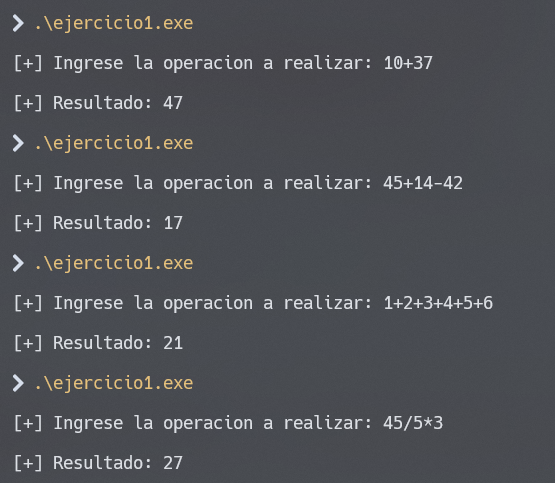
\includegraphics[width=0.8\textwidth,keepaspectratio]{img/ejercicio1.png}
        \end{figure}

        \textbf{Análisis del código:} \\\\
        En el anterior código, presenta una calculadora básica para realizar operaciones matemáticas con una cadena de entrada que contiene hasta seis números y operadores matemáticos (\verb|+|, \verb|-|, \verb|*|, \verb|/|). La clase \texttt{Operacion} define el método \texttt{analizarOperaciones}, que recibe una cadena de texto, analiza los operadores y los almacena dinámicamente en un arreglo. La clase \texttt{NucleoCalculadora} contiene el método \texttt{realizarOperacion}, el cual evalúa la operación matemática entre dos números dependiendo del operador. La clase \texttt{Procesador} se encarga de extraer los números de la cadena, almacenarlos en un arreglo dinámico y procesar las operaciones de manera secuencial usando el método \texttt{realizarOperacion}. Se utiliza manejo manual de memoria con \texttt{new} y \texttt{delete} para los arreglos de números y operadores, garantizando que no haya fugas de memoria mediante el destructor de la clase \texttt{Procesador}.


    \subsection{Ejercicio 2}
        \begin{itemize}
            \item Implementar con punteros una lista doblemente enlazada, utilizar clases o struct. 
        \end{itemize}  
        
        \lstinputlisting[language=C++, caption={ejercicio2.cpp}, numbers=left]{src/ejercicio2.cpp}

        \textbf{Ejecución del ejercicio} \\\\
        Se realizaron las siguientes insercciones:
        \begin{itemize}
            \item lista.insertarFinal(10);
           \item lista.insertarFinal(20);
           \item lista.insertarInicio(5);
           \item lista.insertarInicio(1);
        \end{itemize}
        \begin{figure}[H]
        	\centering
         	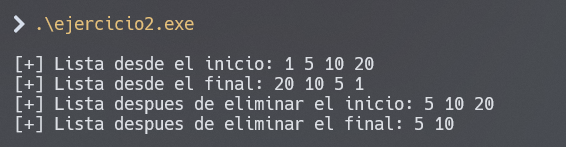
\includegraphics[width=0.8\textwidth,keepaspectratio]{img/ejercicio2.png}
        \end{figure}

        \textbf{Análisis del código:}  \\\\
        En el anterior código, se implementó una lista doblemente enlazada mediante la estructura \texttt{Nodo} y la clase \texttt{ListaDobleEnlazada}. Cada \texttt{Nodo} contiene un valor entero y punteros a los nodos adyacentes (\texttt{siguiente} y \texttt{anterior}). La clase \texttt{ListaDobleEnlazada} maneja dos punteros principales: \texttt{cabeza} y \texttt{cola}, que apuntan al inicio y final de la lista, respectivamente. Los métodos \texttt{insertarFinal} e \texttt{insertarInicio} permiten agregar nodos al final o al inicio de la lista. Las operaciones \texttt{eliminarFinal} y \texttt{eliminarInicio} eliminan los nodos correspondientes, ajustando los punteros de manera adecuada. La lista puede ser recorrida en ambas direcciones con los métodos \texttt{mostrarDesdeInicio} y \texttt{mostrarDesdeFinal}. Finalmente, el destructor libera la memoria de todos los nodos para evitar fugas.
        
\clearpage

\section{Cuestionario}
    \begin{enumerate}
        \item \textbf{¿Qué es la memoria dinámica y para que nos sirve?} \\\\
        La memoria dinámica es un tipo de memoria que se asigna y libera en tiempo de ejecución, en lugar de hacerlo en tiempo de compilación. Esto nos permite reservar espacio en el heap según sea necesario, especialmente útil cuando no sabemos de antemano cuánta memoria necesitaremos, como en el caso de estructuras de datos que pueden cambiar de tamaño (listas, árboles, etc.). Sirve para manejar grandes cantidades de datos de manera flexible y eficiente.
            
        \item \textbf{¿Cuáles son las principales recomendaciones para el uso de la memoria dinámica?} \\\\
        Es importante asegurarse de liberar la memoria asignada dinámicamente una vez que ya no se necesite, utilizando la palabra clave \texttt{delete} o \texttt{delete[]} en C++. Esto evita fugas de memoria, que pueden causar que un programa consuma más memoria de la necesaria. También se recomienda inicializar punteros a \texttt{nullptr} después de liberarlos para evitar el acceso accidental a direcciones de memoria inválidas. 

        \item \textbf{¿Qué sentencias son usadas en C++ para el manejo de memoria dinámica?. ¿Cómo se utilizan?
        } \\\\
        En C++, se usa la sentencia \texttt{new} para asignar memoria dinámica y \texttt{delete} para liberarla. Por ejemplo, \texttt{int *p = new int;} asigna un entero en el heap y devuelve un puntero a esa memoria. Para liberar esa memoria, se usa \texttt{delete p;}. Si es un arreglo dinámico, se utiliza \texttt{delete[] p;}. Es importante usar esto para evitar fugas de memoria.
        
    \end{enumerate}

\begin{comment}
\section{Referencias}
\begin{itemize}			
	\item \url{https://dialnet.unirioja.es/servlet/articulo?codigo=4573315}
\end{itemize}	    
\end{comment}

\end{document}